\section{搬运量约束下的流水优化}
\subsection{完整执行时间模型}
在原图上加入换入换出依赖和地址复用依赖，得到驻留图 $G_R=(V_R,E_R)$。换出须等待本驻留段的全部使用者，换入须等待对应换出，后续使用者须等待换入。若地址被复用，则新驻留段的开始节点等待旧驻留段的释放节点。无换出时，该关系正好退化为题面的释放到申请边。

对给定序列，同一执行单元的前一条指令记为 $h(v)$，实际时间由
\begin{align}
S_v &= \max\left(0,\max_{u:(u,v)\in E_R}F_u,F_{h(v)}\right),\\
F_v &= S_v+c_v,\qquad T=\max_{v\in V_R}F_v
\end{align}
递推得到；不存在前项时相应项取零。管理节点没有独占执行单元。这个模型允许不同单元重叠，但绝不允许绕过缓存复用所需的同步。

\subsection{地址轮换与固定驻留图重排}
最佳适配往往重复使用低地址，即使其他区间暂时空闲，也会增加相邻任务间的物理依赖。地址轮换从上次分配末端继续寻找空闲区间，绕回后再搜索。该操作可能改变碎片和换出次数，因此只有满足 $D\le D_2$ 的方案才保留。初始候选还包括估计最早开始时间和新增缓存量的加权排序，最终都由完整评价模型重新计算。

进一步固定已选方案的所有驻留段顺序及地址关系，仅重新安排执行单元上的指令顺序。首先按已有合法序列逆序计算
\begin{equation}r_v=c_v+\max_{u:(v,u)\in E_R}r_u,\end{equation}
然后维护每个执行单元按 $r_v$ 排序的就绪队列。管理节点就绪后优先处理；操作节点在各队列队首间按最早可开始时间择优，同分取较长下游路径。另比较直接按关键路径择优的规则。由于只改变拓扑序，不改驻留对象、偏移与换出事件，额外搬运量保持不变。重排后按换出实际出现顺序重新编号新增节点，并同步更新配对换入编号，保证文本附件次序一致。

固定驻留图也限制了可搜索空间：保留的物理复用顺序可能排除更优的地址方案。它是可行的局部优化方法，不是同时优化所有物理布局的精确算法。优先队列维护和下游路径计算开销为 $O((N+M)\log(N+M)+|E_R|)$，还需计入构造复用边时扫描缓存单元的开销。

\subsection{优化效果}
\begin{table}[H]\centering\caption{问题三最终结果及相对问题二的时间降低}\small
\begin{tabular}{lrrr}\toprule 计算图 & 搬运量 & 周期 & 降低比例（\%）\\\midrule
Conv\_Case0 & 44766 & 465892 & 1.30 \\
Conv\_Case1 & 75546 & 1044075 & 13.76 \\
FlashAttention\_Case0 & 3620 & 37744 & 20.55 \\
FlashAttention\_Case1 & 32852 & 150499 & 33.38 \\
Matmul\_Case0 & 34944 & 173274 & 10.84 \\
Matmul\_Case1 & 460800 & 1749773 & 2.79 \\
\bottomrule\end{tabular}
\end{table}
\begin{figure}[htbp]\centering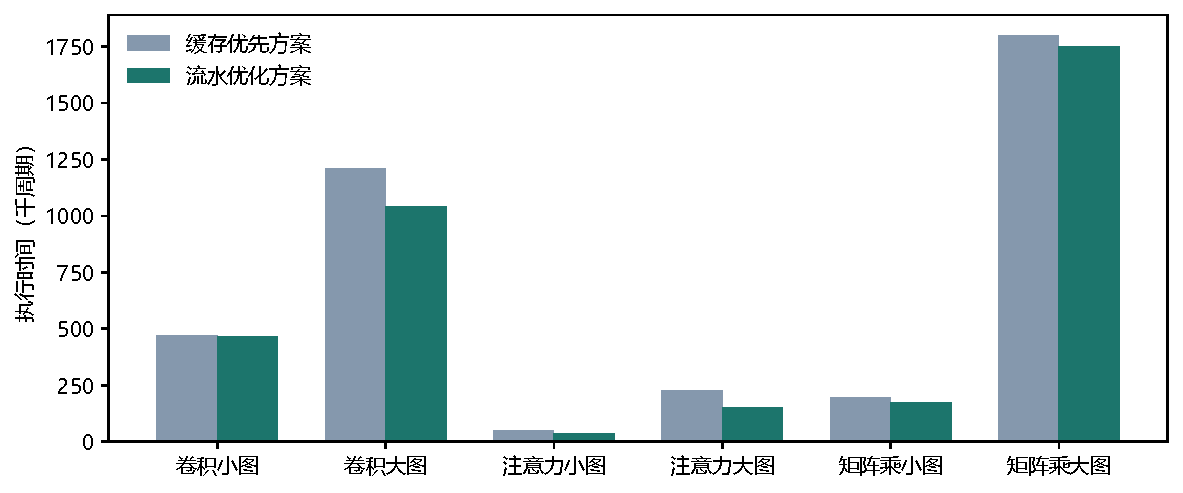
\includegraphics[width=.94\linewidth]{../figures/npu2025/time.pdf}
\caption{缓存优先方案与流水优化方案的执行时间}\label{fig:time}\end{figure}
六个图的搬运量均保持不变，时间改善存在明显差异。注意力大图改善最多，说明该图在既有地址约束下仍有较大的异构执行单元交错空间；卷积小图改善较少，表明仅调整指令顺序的收益有限。该解释基于当前候选表现，不推广为所有同类算子的固定规律。

\begin{figure}[htbp]\centering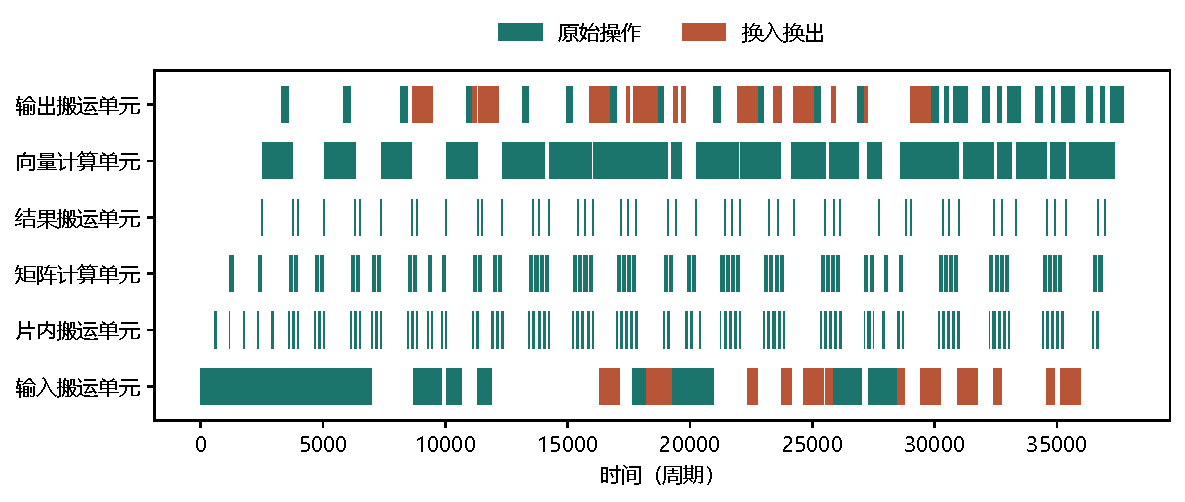
\includegraphics[width=.96\linewidth]{../figures/npu2025/pipeline.pdf}
\caption{注意力小图最终方案的完整执行单元流水}\label{fig:pipeline}\end{figure}
图\ref{fig:pipeline}将原始操作与换入换出分色。空白区间表示相应执行单元等待，竖向重叠表示不同单元同时运行。换出耗时为零的事件不形成可见条块，但仍保留在调度序列及依赖检查中，避免通过图形省略误认为没有换出。

